%\documentclass[letterpaper, 10 pt, conference]{ieeeconf}  % Comment this line out if you need a4paper
%\documentclass[11 pt, onecolumn]{IEEEtran}

\documentclass[10pt]{article}      % Use this line for a4 paper

\usepackage{amsmath,amssymb,euscript,yfonts,psfrag,latexsym,dsfont,graphicx}
\usepackage{bbm,color,amstext,wasysym,parskip,balance}
\usepackage{subcaption}
\usepackage{url}
\usepackage[pdftex,hidelinks]{hyperref}

%\usepackage{amsthm}
%\usepackage{refcheck}
%\usepackage{showkeys}
%\usepackage{epstopdf,hyperref,pdfsync,url}
%\graphicspath{{./},{./figures/},{./Matlab/}}




\newtheorem{thm}{Theorem}
\newtheorem{cor}[thm]{Corollary}
\newtheorem{conj}[thm]{Conjecture}
\newtheorem{lemma}[thm]{Lemma}
\newtheorem{prop}{Proposition}
\newtheorem{problem}[thm]{Problem}
\newtheorem{remark}[thm]{Remark}
\newtheorem{defn}[thm]{Definition}
\newtheorem{ex}[thm]{Example}

\newcommand{\mR}{{\mathbb R}}
\newcommand{\mD}{{\mathbb D}}
\newcommand{\cH}{{\mathcal H}}
\newcommand{\E}{{\mathbb E}}  % this is for expectation -- we can change
\newcommand{\bx}{{\mathbf x}}
\newcommand{\mE}{{\mathbb E}}
\newcommand{\cD}{{\mathcal D}}
\newcommand{\cN}{{\mathcal N}}
\newcommand{\cM}{{\mathcal M}}
\newcommand{\cR}{{\mathcal R}}
\newcommand{\cS}{{\mathcal S}}
\newcommand{\cC}{{\mathcal C}}
\newcommand{\cP}{{\mathcal P}}
\newcommand{\cU}{{\mathcal U}}
\newcommand{\cL}{{\mathcal L}}
\newcommand{\cT}{{\mathcal T}}
\newcommand{\diag}{\operatorname{diag}}
\newcommand{\tr}{\operatorname{trace}}
\newcommand{\f}{{\mathfrak f}}
\newcommand{\g}{{\mathfrak g}}
\newcommand{\range}{\cR}
\newcommand{\rH}{{\rm H}}
  %{\operatorname{range}}
\newcommand{\trace}{\operatorname{tr}}
\newcommand{\argmin}{\operatorname{argmin}}

%\newcommand{\ignore}[1]{}

%\def\spacingset#1{\def\baselinestretch{#1}\small\normalsize}
%\setlength{\parskip}{10pt}
%\setlength{\parindent}{20pt}
%\spacingset{1}

%\newcommand{\mike}{\color{magenta}}
%\newcommand{\mmike}{\color{blue}}
%\newcommand{\jk}[1]{{\color{red}{#1}}}

%\newcommand{\rike}[1]{{\color{red}{#1}}}
%\newcommand{\rike}{\color{red}}

\definecolor{grey}{rgb}{0.6,0.6,0.6}
\definecolor{lightgray}{rgb}{0.97,.99,0.99}

%\IEEEoverridecommandlockouts
%\overrideIEEEmargins

%\renewcommand{\baselinestretch}{0.985}

%\def\spacingset#1{\def\baselinestretch{#1}\small\normalsize}
\setlength{\parskip}{5.3pt}
%\setlength{\parindent}{10pt}
%\spacingset{1}

\setlength{\voffset}{2pt}

\title{FLIR project - modelling noise in bolometer signal}
\author{
Project group (alphabetic order): \and
Carl Ringqvist \texttt{carrin@kth.se} \and
Giampaolo Mele \texttt{gmele@kth.se} \and
H\aa kan Carlsson \texttt{hakcar@kth.se} \and
Johan Karlsson \texttt{johan.karlsson@math.kth.se} \and
M\"arta Barenthin Syberg \texttt{Marta.BarenthinSyberg@flir.se} \and
Olof Runborg \texttt{olofr@nada.kth.se} \and
Per Enqvist \texttt{penqvist@kth.se} \and
Ulf Wållgren \texttt{ujgwallgren@gmail.com}
}

% Comment colours
\usepackage{xcolor}
\newcommand{\gm}[1]{{\color{blue}#1\color{black}}}

\begin{document}


\maketitle

\begin{abstract}
A microbolometer is a device for measuring the power of incident
electromagnetic radiation via the heating of a material with a
temperature-dependent electrical resistance in infrared (IR)
cameras. The change in the resistance is measured with an applied bias
voltage, which yields an current that is fed to an integrator. The
integrator then yields an readout voltage that represents the output
signal of the system. The bias voltage also heats the resistance, and
thus in the uncooled microbolometer system, the bias voltage is only applied
peridically to allow the resistance to cool down. In the camera, an
array of bolometers gives an IR image. Based on the heat equation and
the Stefan Boltzmann law of black-body radiation, there are
mathematical models describing the underlying behavior of the
bolometer, before the readout voltage. We would like to investigate if
the underlying bolometer parameters can be identified using readout
voltage data. Further, we investigate how noise affects the system and
how the models can be modified to account for the noise. A
better understanding of the components (detectors) could potentially
strengthen the capabilities to reduce noise. This report is done in
collaboration with FLIR, based in T\"aby. FLIR develops and produces
cameras for temperature
measurement.

\end{abstract}

\section{Introduction}


\subsection{The IR camera}
Electromagnetic radiation of wavelengths between $700$ nanometer to
$1$ millimeter comprise what is usually referred to as
\textit{infrared light}. Much like the normal camera is able to detect
and display variations of visible light ($400$ nanometers to $700$
nanometers), infrared cameras produce pictures colored
according to the variations in infrared radiation (IR) of a
scene. Since infrared emission from an object is closely related to
its temperature, an IR camera essentially produces a heat map to the
eye, coloring parts of a scene relative to temperature. For instance
in Figure~\ref{fig:cat}, a cat is depicted based on the IR radiation
it emits. Many infrared
cameras are also able to accurately estimate the temperature of an
object in addition to depicting it.


\begin{figure}[h]
\begin{center}
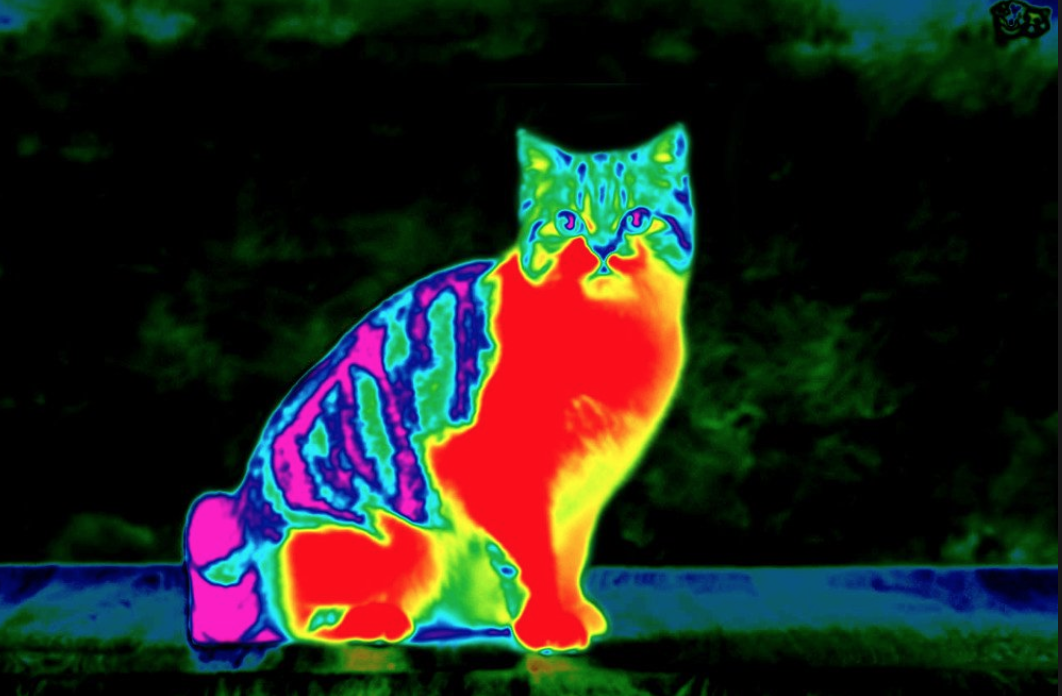
\includegraphics[height=5cm]{gfx/cat.png}
\caption{Infrared picture of a cat sitting on a table during
  night. The warmblooded cat is clearly distinguished from its cold
  surrounding, making the cat visible to the IR camera although not
  visible to the eye. Source:
  https://www.scienceabc.com/}~\label{fig:cat}
\end{center}
\end{figure}

Infrared cameras are used widely within industrial and military
applications, enabling or enhancing tasks such as dark vision, heat
leakage detection, moisture detection, chemical spill leakage
detection and firefighting. An overview about different devices
together with a catalog can be found in~\cite{flir_handbook}. There
exist mainly two types of techniques for infrared cameras: thermal
detectors and quantum detectors. We will here focus solely on thermal
detectors, and especially the \textit{uncooled bolometer}. A bolometer consists of a plate (pixel)
made of metal or semiconductor material, which for instance could be a mixture of
silicon nitride and vanadium oxide. This plate suspended in the air
via two supporting legs that is connected to a substrate. The
supporting legs are also connected to a voltage
source. The structure is depicted in Figure~\ref{fig:structure}. Incoming infrared radiation is focused via a lens to the
plate, causing it to be heated, which in turn alters its
resistance. This change in resistance can be measured through an
input voltage and the resulting current is a function of the strength
of the incoming infrared radiation and hence
the temperature of the emitting scene.

\begin{figure}[h]
\begin{center}
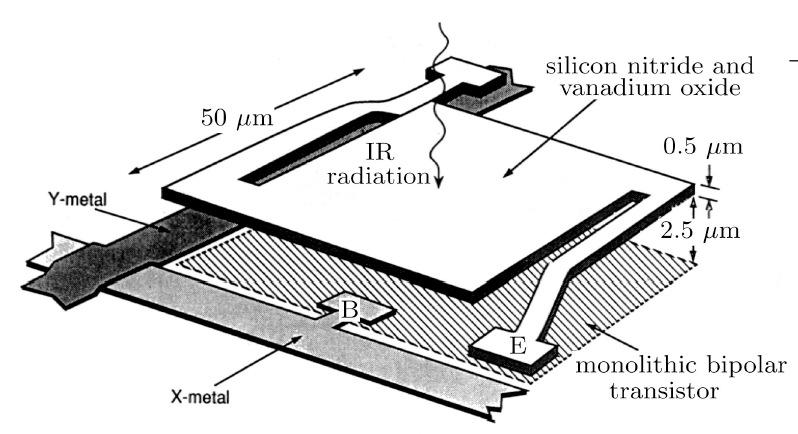
\includegraphics[height=5cm]{gfx/pixel1.png}
\caption{Physical structure of the bolometer~\cite{xiu2010research}.}~\label{fig:structure}
\end{center}
\end{figure}

\subsection{Project description}

The project aims to establish a mathematical relationship between the
temperature of an object and the resulting bolometer signal. Briefly,
the incoming radiation of an object, described by the Stefan-Boltzmann
law, heats up the bolometer, which can be described by the heat
equation. The applied voltage is used to measure the change in
resistance due to the temperature change. More precisely, the
output signal is a voltage from an integrator, that can be used to
retrieve the change in the resistance and thus via the heat equation
and the Stefan-Boltzmann law the temperature of the target. An explicit
description of the output signal is given in
Section~\ref{sec:model_disc}.


%By solving the ODE's numerically, we can get the output signal $v_s$ as a deterministic function of $T_o$. In reality however, the output signal $v_s$ is noisy. The project aims to incorporate noise into the model in a manner consistent with data and experience. A good model of the noisy signal might for example enable an efficient filtering that reduces noise.

In reality however, the output signal is noisy. The project aims to incorporate noise into the model in a manner consistent with data and experience. A good model of the noisy signal might for example enable an efficient filtering that reduces noise. The project's aim is to investigate how a noisy input signal effects the output signal.

More precisely in this project we:
\begin{itemize}
 \item simulate the read-out signal of the bolometer by solving the differential equations modeling the problem,
 \item reproduce numerical simulations that fits with empirical experiments,
 \item model and analyze the noise in the differential equations,
 \item reproduce numerical simulations (with noise) that fits with empirical experiments.
\end{itemize}

%%% Local Variables:
%%% mode: latex
%%% TeX-master: "main"
%%% TeX-PDF-mode: 1
%%% TeX-PDF-via-dvips-ps2pdf: 1
%%% End:
			% Carl
\setlength{\belowcaptionskip}{-15pt}
\setlength{\abovecaptionskip}{0pt}
\section{Model and discretization} \label{sec:model_disc}

Each pixel of an IR camera can be modeled as the circuit in Figure~\ref{fig:circuit}.
\begin{figure}[ht]
 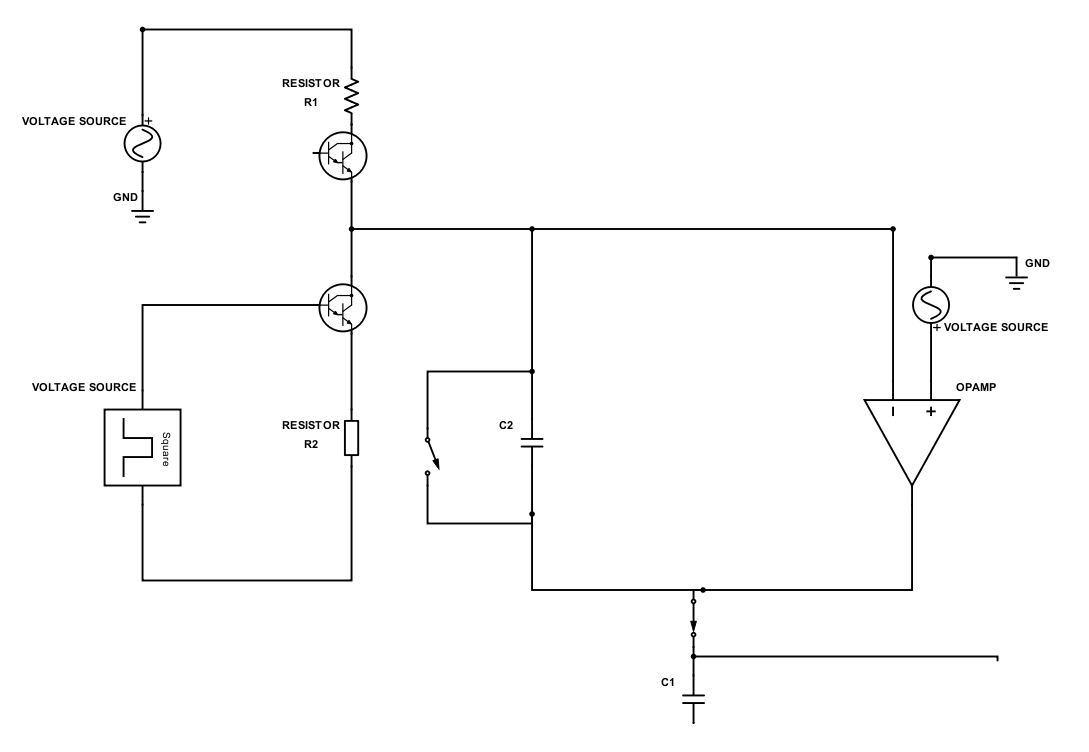
\includegraphics[scale=0.31]{gfx/circuit.png}
\caption{Circuit schematic that model a pixel of the IR camera generated with \url{https://www.digikey.com/schemeit}.}
\label{fig:circuit}
\end{figure}
More precisely the bolometer corresponds to the resistor R2. 

The pixel of the IR camera works as follow: a bias voltage is applied as square signal. The voltage is a piecewise constant function defined as 
\begin{align} \label{eq:Vb}
 V_b(t)&=\begin{cases} v_b & n t_f < t < n t_f + t_i \\
 0 &\mbox{ otherwise.} 
 \end{cases} && n \in {\mathbb N}
\end{align}
The readout signal is the voltage $V_{samp}$ across the capacitor C2 that we can express, by using the Kirchhoff's law, as
\begin{align} \label{eq:Vsamp_def}
 V_{samp} = 
 \frac{1}{\tilde C} \int_{n t_f}^{n t_f + t_i} \left( \frac{V_0}{R_S} - \frac{V_b(s)}{R(T(s))} \right) ds + E
\end{align}
where $R(T)$ is the value of the resistance of R2 as function of the temperature and $\tilde C$ is the capacitance of C2. In \cite{xiu2010research} this is modeled as $R(T)=R_S e^{\alpha(T-T_s)}$ where $\alpha$ is a constant that depends on the material of the bolometer. Clearly, in order to compute this integral, we need to know the temperature as function of the time. This relation is described  by the  \emph{heat balance equation} \eqref{eq:heat_balance_equation}.

The output signal can therefore be simulated in the following way. We set an initial temperature $T_0$ for the bolometer and solve the heat balance equation~\eqref{eq:heat_balance_equation}. Then we compute the integral describing the readout signal~\eqref{eq:Vsamp_def}.


\subsection{Illustrative example} \label{sec:example}
A reasonable and realistic simulation of the bolometer response can be obtained by solving the equations~\eqref{eq:heat_balance_equation}-\eqref{eq:Vsamp_def} with the parameters and coefficients given in Table~\ref{tab:par_coeffs_example}. Moreover we have set $T_0=T_s$, $P_t=A_s \sigma (T_0+10)^4$ and $P_s=A_s \sigma T_s^4$.


The solution of~\eqref{eq:heat_balance_equation} is illustrated in Figure~\ref{fig:solution_heat_balance_eq}. In the phase when the bias voltage is active, usually referred as \emph{integration time}, the temperature of the bolometer rises of circa $3K$. This is due to the fact that the current flowing through a component causes its overheat. When the bias voltage is not active, the temperature of the bolometer drops of circa $3K$, therefore we refer to this phase as \emph{cooling time}. See Figure~\ref{fig:solution_heat_balance_eq_splitted} for the illustration this such phenomena. The readout is illustrated in Figure~\ref{fig:Vout}. 

\begin{figure} 
 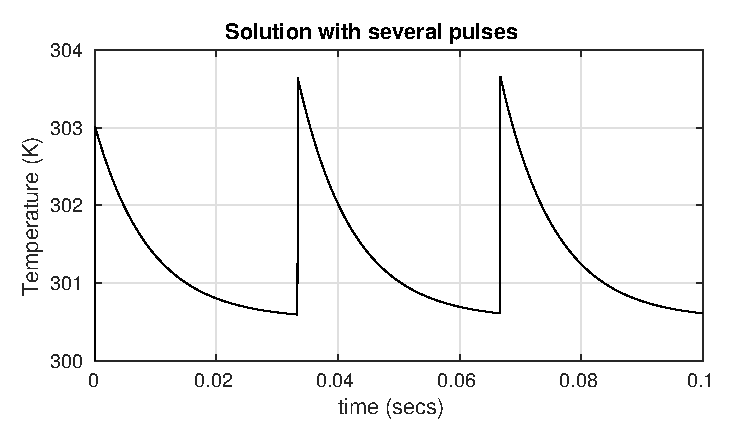
\includegraphics[scale=0.9]{gfx/fig1_several_pulses.eps} 
 \caption{Solution to the heat balance equation~\eqref{eq:heat_balance_equation}.}
 \label{fig:solution_heat_balance_eq}
\end{figure}
\begin{figure} 
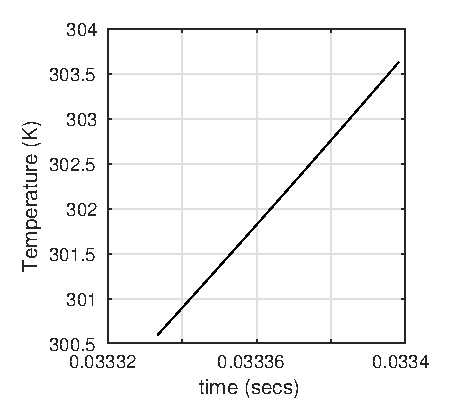
\includegraphics[scale=0.9]{gfx/fig1_int_time.eps} 
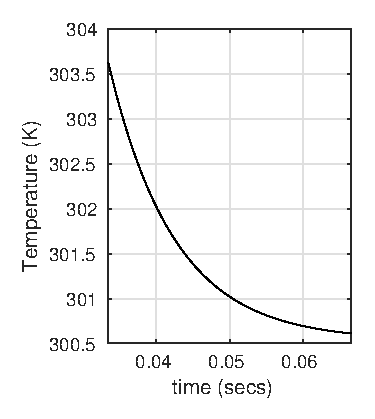
\includegraphics[scale=0.9]{gfx/fig1_cooling.eps}
\caption{Solution to the heat balance equation~\eqref{eq:heat_balance_equation} during the integration time $V_b>0$, and during the cooling time $V_b=0$. }
\label{fig:solution_heat_balance_eq_splitted}
\end{figure}
\begin{figure}
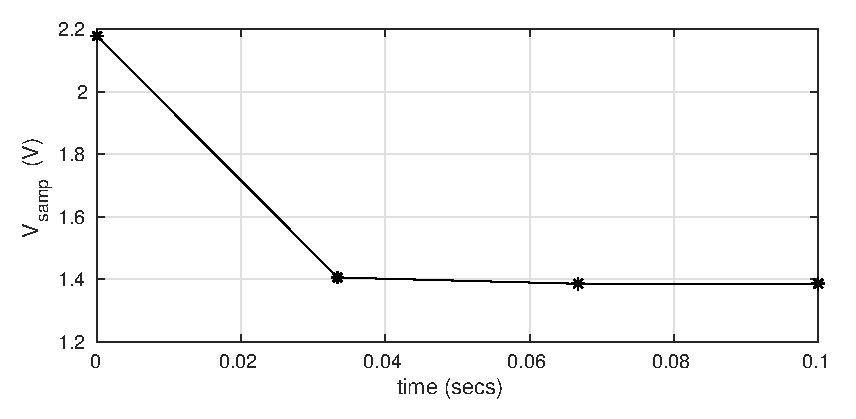
\includegraphics[scale=0.9]{gfx/fig1_Vout_several_pulses.eps} 
\caption{Readout voltage~\eqref{eq:Vsamp_def}.}
\label{fig:Vout}
\end{figure}

As we can see in Figure~\ref{fig:solution_heat_balance_eq}-\ref{fig:solution_heat_balance_eq_splitted}, the temperature of the bolometer does not only depend on the incoming IR radiation, namely the temperature of the object we are observing, but also on the bias voltage. In order to mitigate this phenomena, the frame-time $t_f$ is set much larger than the integration time $t_i$ to avoid overheat the bolometer. In particular the function temperature $T$ oscillates in the time (after very few pulses) around the temperature due to the incoming IR radiation. This also reflects in the readout, since $V_{samp}$ becomes constant, i.e., the bolometer has cached the temperature of the observed object.

\begin{center}
\begin{table}[]
\centering
\caption{Parameters and coefficients used in Section~\ref{sec:example}}
\label{tab:par_coeffs_example}
\begin{tabular}{|c|cr|c|cr|}
\hline
 $t_i$ 		& $65$ 		& $  \mu sec$ 		& $\alpha$  	&    	$-0.02$	&			\\
\hline 
 $tf$ 		& $1/30$ 	& $  sec$ 	 	& $e$ 		&    	$0.8$ 	&			\\
\hline 
 $R_S$ 		& $800 $ 	& $  k \Omega$ 		& $A$ 		&    	$17  $ 	& $ \mu m$ (square)	\\
\hline 
 $T_s$		& $300 $ 	& $  K$ 	 	& $A_s$ 	&    	$17  $ 	& $ \mu m$ (square)	\\  
\hline 
 $G_{leg}$	&  $250 $ 	& $   \mu W K^{-1}$	& $\tilde C$ 	&	$4$ 	& $   p F$		\\   
\hline 
 $C$		&  $25 $ 	& $   n J K^{-1}$ 	& $V_0$		& 	$3.1$ 	& $   V$		\\
\hline 
 $v_b$		& $3 $ 		& $   V$		& $E$		& 	$2$ 	& $   V$		\\
\hline 
\end{tabular}
\end{table} 
\end{center}

\subsection{Numerical methods for simulating the bolometer}
The output signal can be simulated by setting an initial temperature for the bolometer and by solving the heat balance equation~\eqref{eq:heat_balance_equation}. The readout $V_{samp}$ corresponds to the integral~\eqref{eq:Vsamp_def} that can be approximated with any numerical integration algorithm such as Riemann sum, trapezoidal rule, etc. The equation~\eqref{eq:heat_balance_equation} cannot be solved naively with a numerical scheme for ODE described, e.g., in \cite{mattheij1996ordinary,ascher1998computer}. Namely, any \texttt{matlab} ODE solver is not capable of solving~\eqref{eq:heat_balance_equation}. This is due to the fact that the function $V_b(t)$ (bias voltage), defined in~\eqref{eq:Vb}, has a very fast variation. The strategy for effectively solve the problem consists in splitting the domain in sub-domains where $V_b(t)$ is constant. 

Assume that we want to solve~\eqref{eq:heat_balance_equation} for $0 \le t \le m t$ for a fixed $m \in \mathbb{N}$, namely we want $m$ pulses. The time domain can be split as
\begin{align*}
 [0, m t_f] = \bigcup_{k=0}^{m-1} (I_k \cup J_k)
\end{align*} 
where $I_k=[k t, k t_f+t_i]$ and $J_k = [k t_f + t_i, (k+1)t_f]$. 
We set $T_0(0):=T_0$ and for $k=1, 2, \dots$, we solve the ODE in $I_k$
\begin{align} \label{eq:heat_balance_equation_seq_bias}
& C\frac{dT_{k+1}}{dt}=\frac{v_b^2}{R(T_{k+1})}+\epsilon_e(P_t+P_s -2A\sigma T_{k+1}^4)-G_{leg}(T_{k+1}-T_s) \ , \ t \in I_k \nonumber \\
& T_{k+1}(kt_f)=T_{k}(kt_f)&
\end{align}
we set $\alpha:=T_{k+1}(kt_f+t_i)$ and we solve the ODE in $J_k$
\begin{align} \label{eq:heat_balance_equation_seq_no_bias}
& C\frac{dT_{k+1}}{dt}=\epsilon_e(P_t+P_s -2A\sigma T_{k+1}^4)-G_{leg}(T_{k+1}-T_s) \ , \ t \in J_k \nonumber \\
&T_{k+1}(kt_f+t_i)=\alpha_{k+1}	
\end{align}
The solution $T(t)$ of~\eqref{eq:heat_balance_equation} is obtained by gluing the functions $T_j(t)$, i.e., 
\begin{align*}
 T(t) = 
 \begin{cases}
  T_0(t) & t \in I_0 \cup J_0	\\
  T_1(t) & t \in I_1 \cup J_1	\\
	 & \vdots 		\\
  T_1(t) & t \in I_k \cup J_k	\\
	 & \vdots		\\
  T_m(t) & t \in I_m \cup J_m	\\
 \end{cases}
\end{align*}
In conclusion, the solutions of the ODEs~\eqref{eq:heat_balance_equation_seq_bias}-\eqref{eq:heat_balance_equation_seq_no_bias} can be approximated with any numerical scheme such us Euler method, Runge--Kutta, etc. We did not observe any difficulty in solving these equations and we chose the explicit Euler method as solver since this can easily be extended to the noised model (stochastic differential equation) that we will introduce in the next section.  

		% Giampaolo
\section{Model with noise and discretization}

There are several sources of noise in a micro-bolometer setup:
\begin{itemize}
\item Thermal noise in the resistances,
\item Flicker noise in resistances,
\item Burst noise,
\item Thermal fluctuations in the bolometer temperature,
\item Noise in incident IR radiation,
\item Noise in read out circuits.
\end{itemize}

In this report we shall only consider the first two types of noises,
thermal and flicker noise in resistances.

\subsection{Thermal noise}

Any resistance with a temperature $T$ above zero, will cause the
charge carriers in the material to fluctuate. The fluctuations are
independent of each other, and will generate a current with a
voltage. This phenomenon is referred to as thermal noise, but is also
known as white noise and Johnson noise. This type of noise was first
discovered by the Swedish engineer John
B. Johnson~\cite{PhysRev.32.97}, and his colleague Harry Nyquist, also
Swedish, provided a theory for the noise based on statistical
physics\cite{PhysRev.32.110}. One of the characteristics of the noise,
is the flat power spectrum for all most all frequencies, which is also
characteristic for white light.

In electrical circuits, thermal noise is commonly modeled as an additional
power source in series with the resistance, see Figure~\ref{fig:johnsonEquivalentNoise}.
\begin{figure}
  \centering
  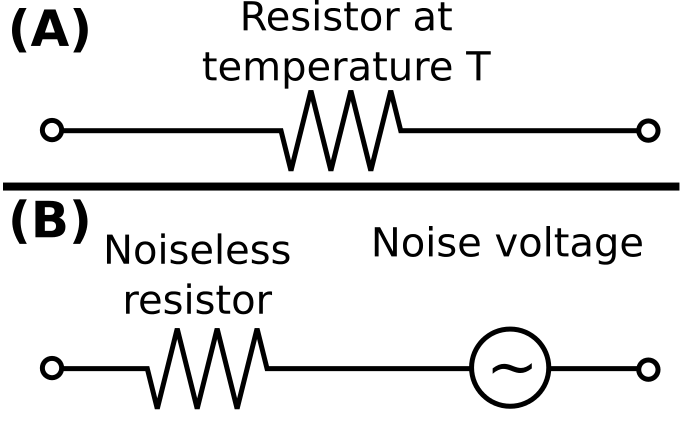
\includegraphics[width=0.5\textwidth]{gfx/JohnsonNoiseEquivalentCircuits.png}
  \caption{Equivalent model for thermal noise in a resistor.}~\label{fig:johnsonEquivalentNoise}
\end{figure}
Due to the random nature of the additional power source, it is not
possible to predict the instantaneous voltage produced, but instead the
average behavior. Nyquist\cite{PhysRev.32.110} found that the power
spectrum of thermal noise to be
\begin{equation}
  \label{eq:power_spectrum_white_noise}
  S(f) = 4 k_B T R,
\end{equation}
where $k_B$ is the Boltzmann constant, $T$ is the temperature of the
resistance, and $R$ is the resistance. The total contribution of the
noise source is then calculated by summing up the contribution from
each frequency component.
\begin{equation}
  \label{eq:2}
  \E \left[ V^2 \right] = \int_B S(f) \mathrm(d) f,
\end{equation}
where $B$ is the bandwidth of the circuit.

% The mean square square voltage o

A statistical model commonly used to white noise is a stationary stochastic
process where the auto-correlation function is
\begin{equation}
  \label{eq:autocorrelation_white_noise}
  R(s,t)={\frac {\operatorname {E} [(X_{t}-\mu _{t})(X_{s}-\mu
      _{s})]}{\sigma _{t}\sigma _{s}}} =
  \begin{cases}
    \sigma_{t}^2 , \quad t = s, \\
    0 , \quad t \neq s
  \end{cases}
\end{equation}
meaning that the process is uncorrelated in time. A distribution that
can be used for this process is the Gaussian distribution
$\mathcal{N}(0, \sigma)$.

\subsection{Flicker Noise}\label{sec:flicker-noise}

Another type of noise source that exists in circuits is flicker
noise, or also known as low frequency noise, 1/$f$ noise or pink noise. The power
spectrum of the Flicker noise is
\begin{equation}
  \label{eq:power_spectrum_flicker_noise}
  S(f) \propto \frac{k}{f^{\alpha}}.
\end{equation}
where $\alpha \in [0.5, 1.5]$ and $k$ is a material constant.

One explanation of the occurrence of the flicker noise in resistors is
that the charge carriers get trapped in capture sites of the
conductor, and are then released with variable rates. This was first
explained by Schottky for flicker noise in vacuum tubes~\cite{PhysRev.28.74}.

To generate the flicker noise in simulation there are several methods
available, listed in~\cite{381848} and~\cite{Stoyanov_2011}.

\subsection{Noise model and simulation scheme}

To compensate for the noise in the read-out circuit, one first has to
determine how noise enters the differential equation governing the
behavior of the system. The simplest possible solution is of course to
add a noise term of a normally distributed character to the left hand side
in Equation~\eqref{eq:heat_balance_equation}, rendering the theory for
diffusion processes readily available. More precisely we rewrite
Equation~\eqref{eq:heat_balance_equation} on the form of a continuous
time stochastic process for variable $T(t)$, i.e.,
\begin{align} \label{eq:continuous_time stochastic_process}
 dT&= \mu(T,t)dt  + K(T,t)dW \\
 T(0)&=T_s	\nonumber
\end{align}
where $K$ and $\mu$ are functions describing the fluctuations of the temperature
increment and the drift in the temperature increment,
respectively. The random variable $W$ denotes a Wiener process, i.e.,
$W \sim N(0, dt)$. Thus, Equation~\eqref{eq:heat_balance_equation} is
reformulated to the form of Equation~\eqref{eq:continuous_time
  stochastic_process} and the function $K$ is chosen according to
the following heuristic.
We expect the noise in the output to be the cause of resistor fluctuations.
Motivated by the setup for Figure~\ref{fig:johnsonEquivalentNoise}, we thus redefine the voltage over
the bolometer resistance as
\begin{equation}
  \label{eq:randomvariable_transformation}
  V \rightarrow V_0 + \Delta V,
\end{equation}
where $V_0$ is the noise-less resistance over the voltage, and $\Delta
V$ is a random variable representing the random fluctuations in the
voltage.

We thus want noise to enter the heat equation in Equation~\eqref{eq:heat_balance_equation}
roughly as
\begin{equation}
  \label{eq:heat_balance_equation_noise}
  C\frac{dT}{dt}=\frac{(V_b(t) + \Delta V)^2}{R(T)}+ f(T),
\end{equation}
where $\Delta V$ is the added noise term, accounting for the
fluctuations in the resistance $R(T)$ and $f(T)$ are the other terms
in Equation~\eqref{eq:heat_balance_equation}.
Expanding the square we get the equation
\begin{equation}
  \label{eq:heat_balance_equation_noise_SDE1}
  C\frac{dT}{dt}=\frac{1}{R(T)} (V_b^2(t) + 2 V_b(t) \Delta V + (\Delta V)^2) + f(T),
\end{equation}
If the squared noise term is negligible in the limit, we are left with
\begin{equation}
  \label{eq:heat_balance_equation_noise_SDE2}
  C\frac{dT}{dt}=\frac{1}{R(T)} (V_b^2(t) + 2 V_b(t) \Delta V  ) +
  f(T) = \frac{V_b^2(t)}{R(T)} + f(T) +  \frac{2 V_b(t) \Delta V}{R(T)}.
\end{equation}
Thus, identifying the terms Equation~\eqref{eq:continuous_time stochastic_process} and Equation
\eqref{eq:heat_balance_equation_noise_SDE2}, yields that the drift
function is
\begin{equation}
  \label{eq:drift_function}
  \mu(T,t) = \frac{1}{C} \left( \frac{V_b^2(t)}{R(T)} + f(T) \right),
\end{equation}
and
\begin{equation}
  \label{eq:variance_function}
  K(T,t)dW = \frac{2 V_b(t) \Delta V}{CR(T)}.
\end{equation}
If we assume that $\Delta V$ is normally distributed with $\Delta V
\sim N(0, \sigma^2 dt)$, where $\sigma$ is a parameter to be calibrated or
physically motivated, then
\begin{equation}
  \label{eq:variance_function}
  K(T,t) = \frac{2 V_b(t) \sigma }{CR(T)}.
\end{equation}
The noisy heat development can now be simulated
in a well defined setting, with the dynamics independent of step size $\Delta t$:
\begin{align} \label{eq:heat_balance_equation_noise_discr}
 CT_{i+1}&=\left(\frac{V_b(t_{i})^2}{R(T_{i})}+\varepsilon(P_t+P_s -2A_s \sigma T_i^4)-G_{leg}(T_i-T_s)\right)\Delta t + \frac{2 V_b(t_i) \sigma \sqrt{\Delta t}}{R(T_{i})} W_i \\
 T(0)&=T_s	\nonumber
\end{align}

where $W_i \sim N(0,1)$.


%%% Local Variables:
%%% mode: latex
%%% TeX-master: "main"
%%% TeX-PDF-mode: 1
%%% TeX-PDF-via-dvips-ps2pdf: 1
%%% End:
 	% Håkan Carlsson
\section{Numerical experiments}

In order to test that the model makes sense from a physical
perspective, simulation experiments have been conducted. Expertise
from FLIR has provided metrics against which outputs from the model
has been benchmarked, along with suggestions for electronic design
experiments. Below the resulting experiments are presented along with
benchmarks if applicable.


\subsection{Solution with noisy model}
For the parameter $\sigma$, we set as a baseline
\begin{align}
\sigma = \sqrt{(4KT_sR(T_s))}
\end{align}
where  $K$ is the Boltzmann constant. This value is of order $1e^{-7}$
and is possible to motivate from a physical perspective. A detailed
explanation can be found in~\cite{WOOD199743}.

We will however amplify or diminish $\sigma$ depending on our needs
with a constant $d$. Thus we will use
\begin{align}
\sigma = d \sqrt{(4KT_sR(T_s))}
\end{align}

Plots from running the temperature simulation and succeeding
integrator with the noisy scheme outlined in
Equation~\eqref{eq:heat_balance_equation_noise_discr} are shown
in Figure~\ref{fig:noisysol}. We see that the difference from the
deterministic solution is marginal, even with amplified noise.

\begin{figure}
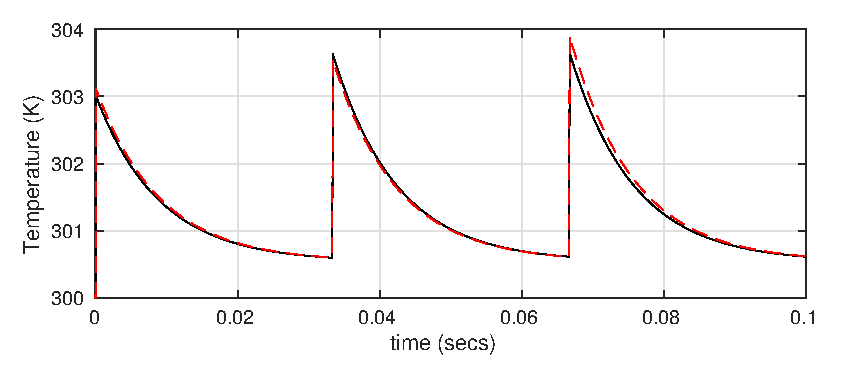
\includegraphics[scale=0.9]{gfx/sol_several_pulses_noise.eps}
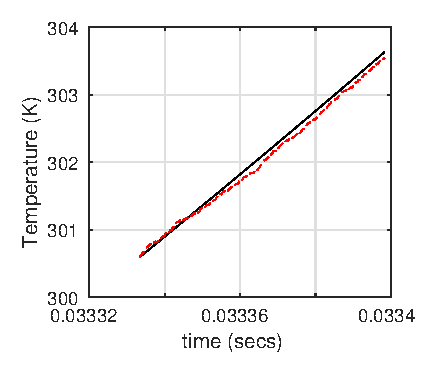
\includegraphics[scale=0.9]{gfx/sol_int_time_noise.eps}
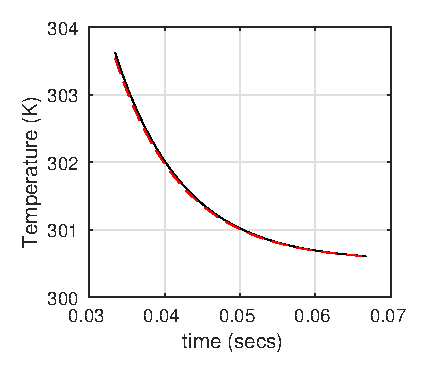
\includegraphics[scale=0.9]{gfx/sol_cooling_noise.eps}
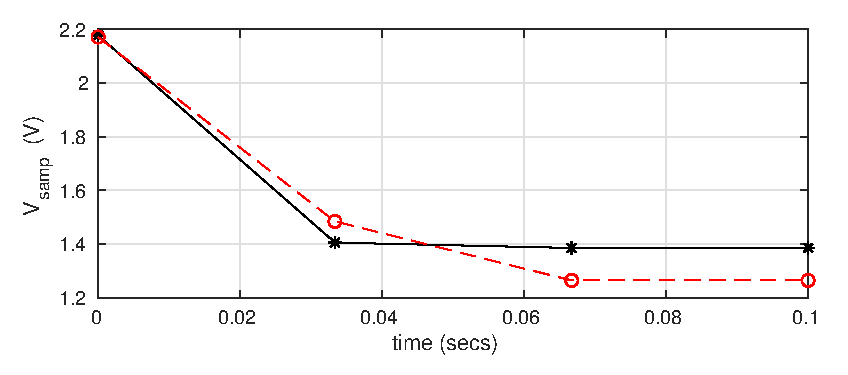
\includegraphics[scale=0.9]{gfx/Vout_several_pulses_noise.eps}
\caption{Temperature and output signal development over time for
  $d=100$. Red: Noisy solution, Black: Deterministic solution}
\label{fig:noisysol}
\end{figure}


\subsection{Investigating model accuracy as function of $\sigma$}
The model accuracy can be measured with the Noise Equivalent Temperature Difference (NETD), which has form
\begin{align}
\mbox{NETD} = \frac{std(V(T, \sigma))}{V(T+1,0)-V(T,0)}
\end{align}
It compares the standard deviation of the noisy output signal at temperature $T$ with the difference in a deterministic signal when heating the observed object
from $T$ to $T+1$. In other words, a large NETD indicates that the noise in the output is too large to detect a change of 1 degree in the observed object.
Figure~\ref{fig:NETD_over_sigma} depicts NETD over $\sigma$ at $T=300$. At this temperature, FLIR has estimated NETD to 20 mK.
This knowledge lets us solve $\sigma$ from the graph, resulting in a value of around $7e^{-6}$.
\begin{figure}[H]
 \begin{center}
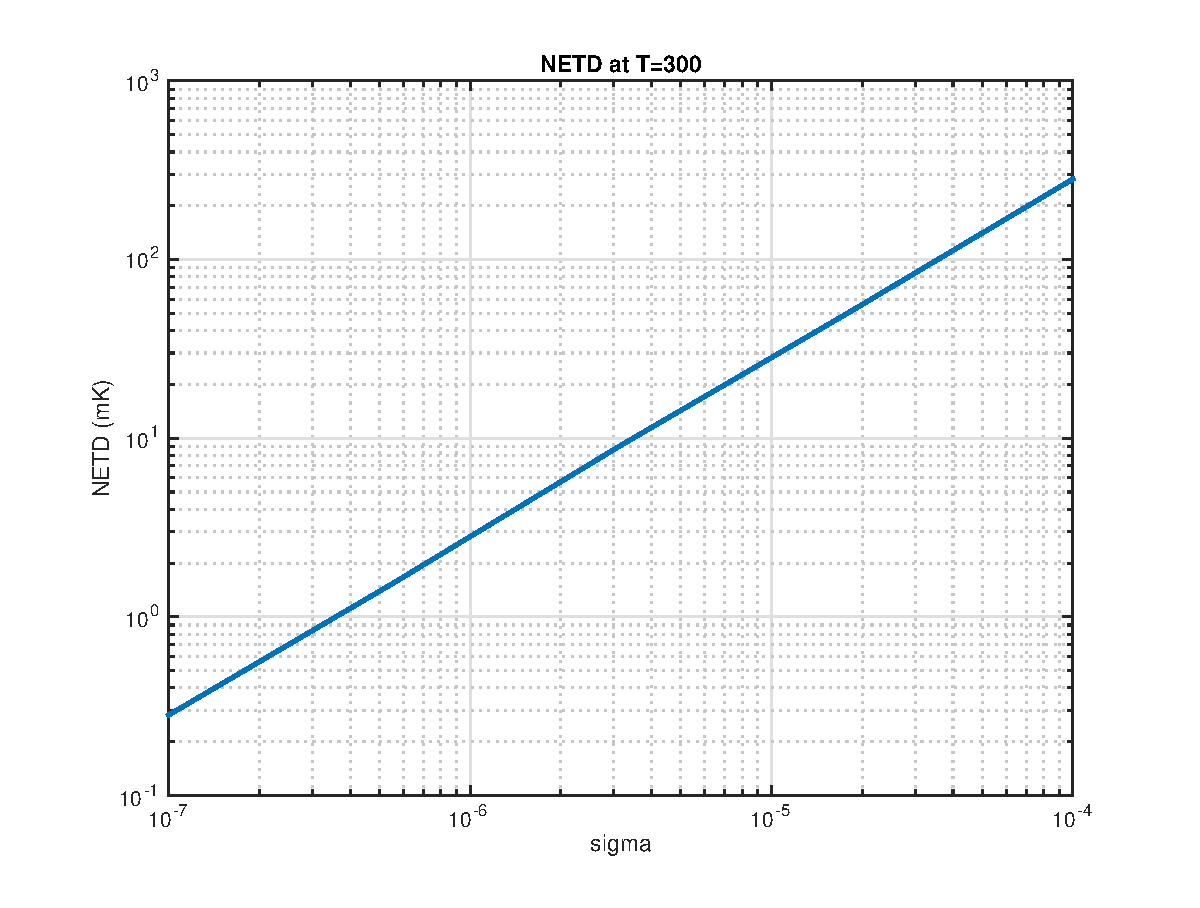
\includegraphics[scale=0.9]{gfx/NETD_as_function_of_sigma.eps}
  \caption{NETD as function of $\sigma$}
  \label{fig:NETD_over_sigma}
  \end{center}
\end{figure}

\subsection{Noise dependence on integration time}
Since measurements are collected only during integration time, a larger integration time on one hand acts to increase the measurement time-span and hence the
reliability of the measurement. On the other hand, a larger integration time infers more substantial heating of the thermistor, resulting in increased noise. It is therefore
of interest to investigate how the output noise depends on the integration time. In Figure~\ref{fig:std_over_time}, signal standard deviations for different frame rates
are plotted against simulations of different integration times. The curve grows approximately as $t^{3/2}$. FLIR has estimated the curve to grow approximately as $t^{1/2}$, indicating
our model is growing at too fast speed. This same peculiarity might explain that the plot of NETD over integration time is increasing, contrary experience at FLIR suggesting
a decreasing NETD-curve.
%\begin{figure}[H]
%    \centering
%    \subfloat[label 1]{{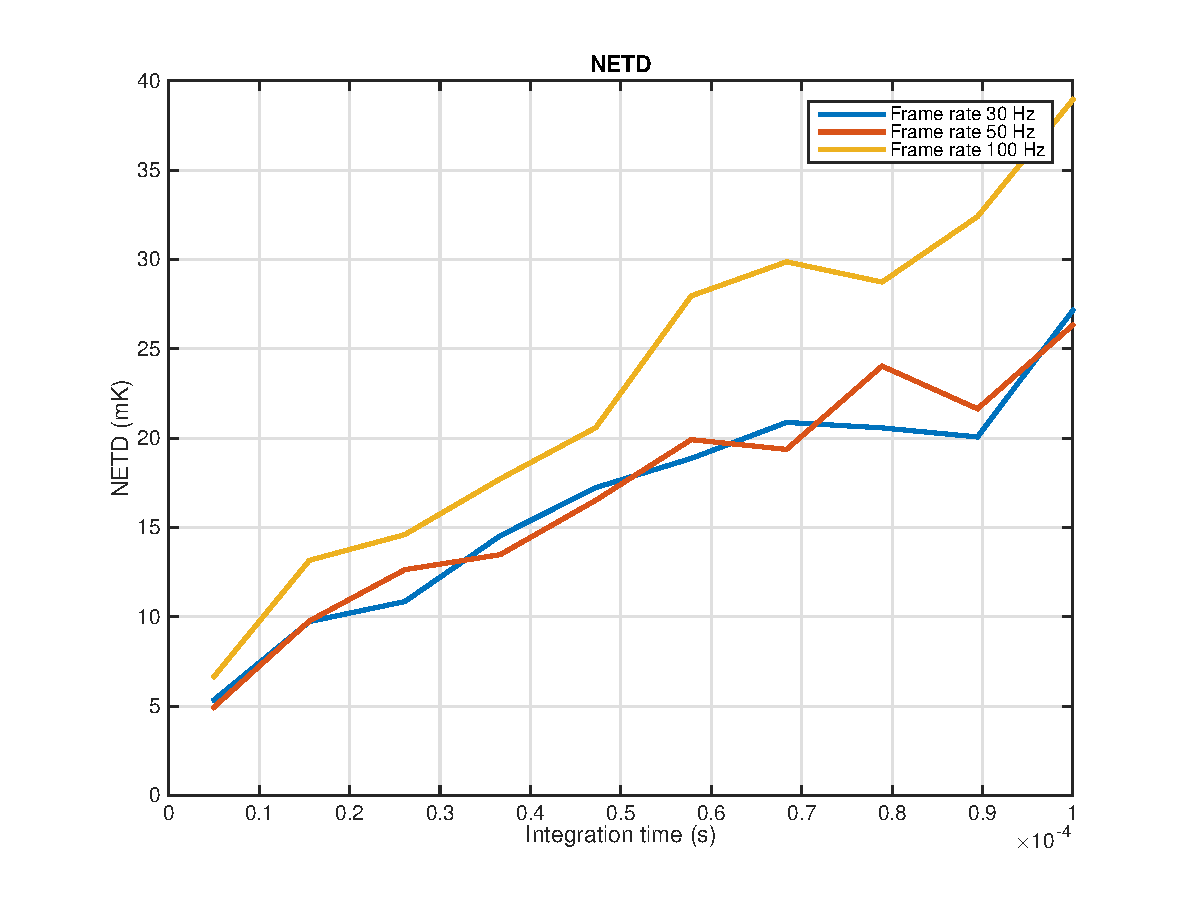
\includegraphics[width=5cm]{gfx/NETS_Function_of_Integration_Time.eps} }}
%    \qquad
%    \subfloat[label 2]{{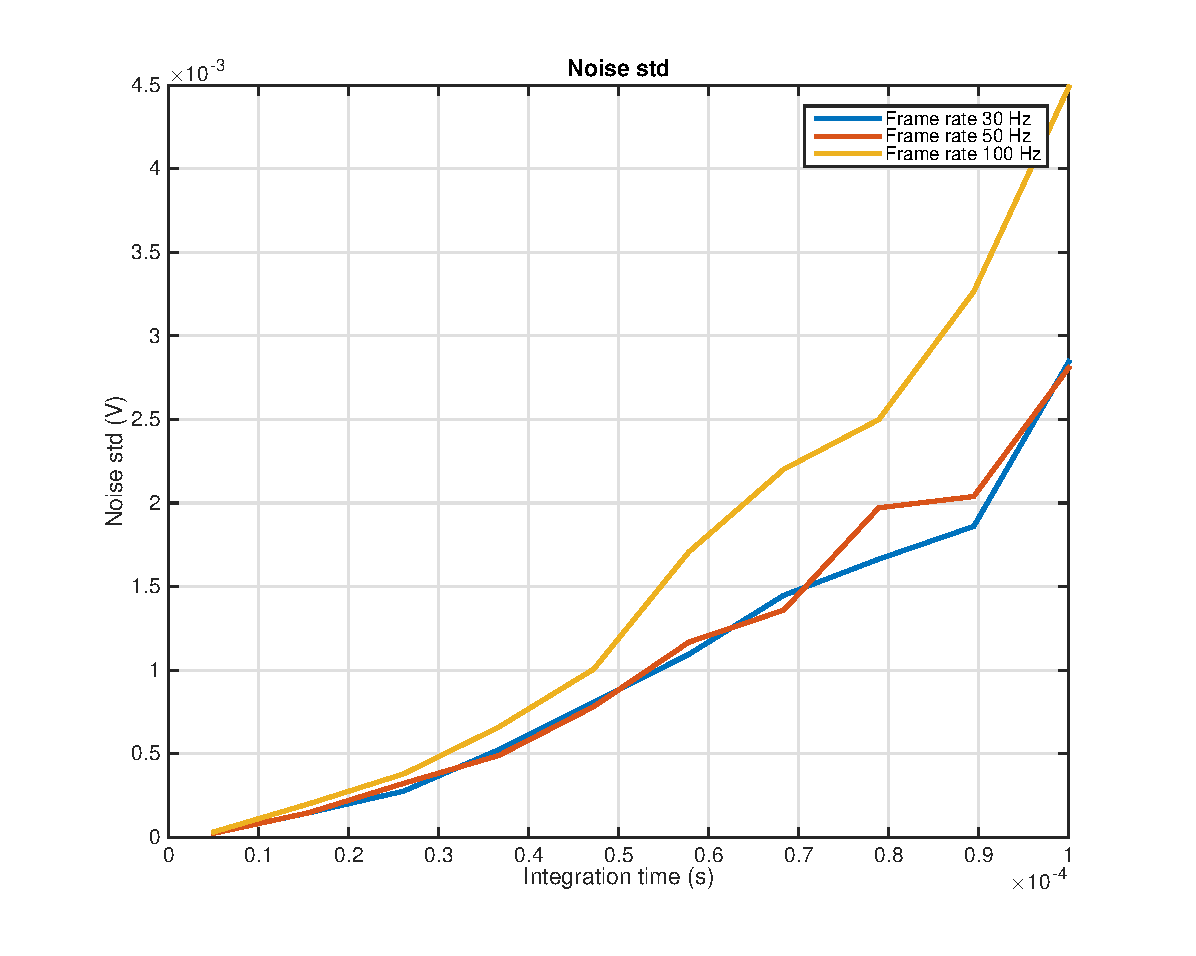
\includegraphics[width=5cm]{gfx/STD_Function_of_Integration_Time.eps} }}
%  \caption{Output standard deviation over integration time}
%  \label{fig:std_over_time}
%\end{figure}
\begin{figure}[H]
 \begin{center}
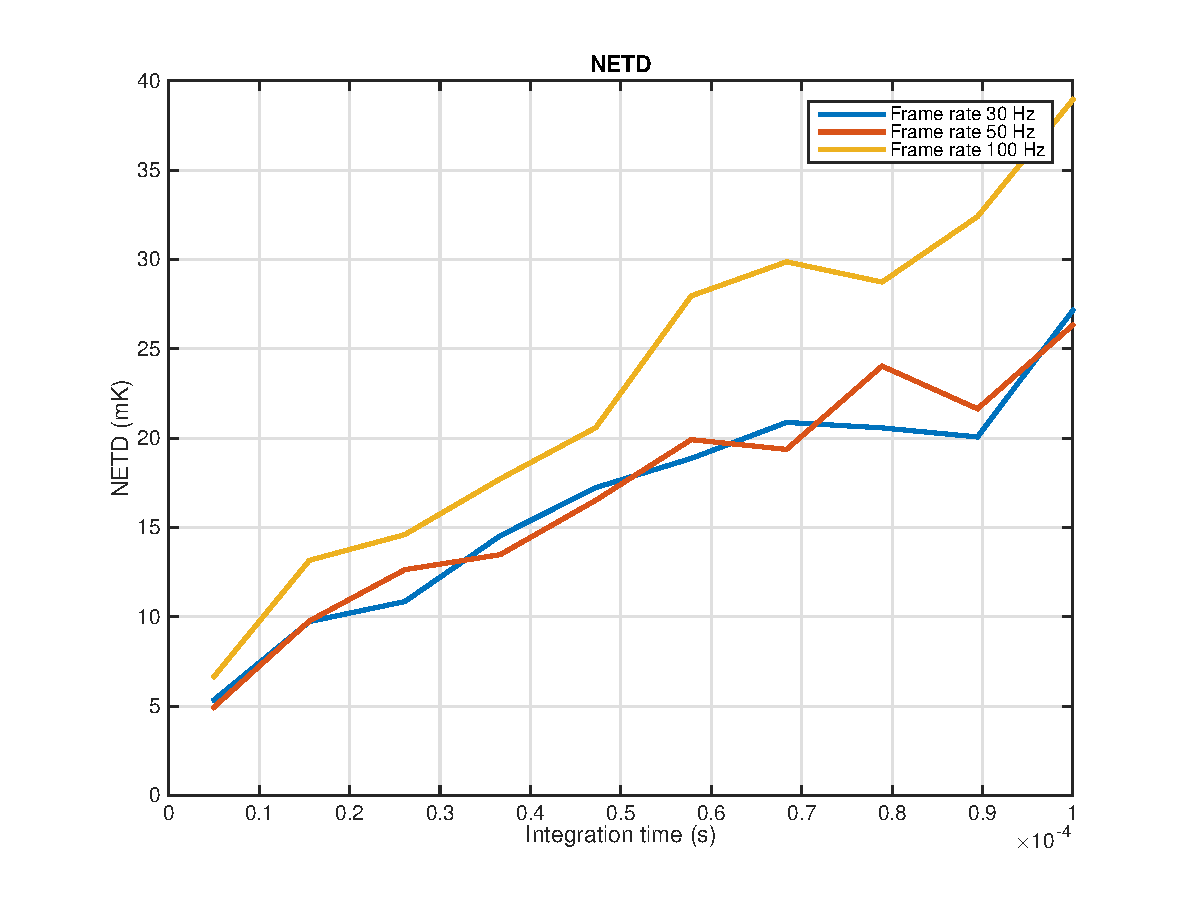
\includegraphics[scale=0.8]{gfx/NETS_Function_of_Integration_Time.eps}
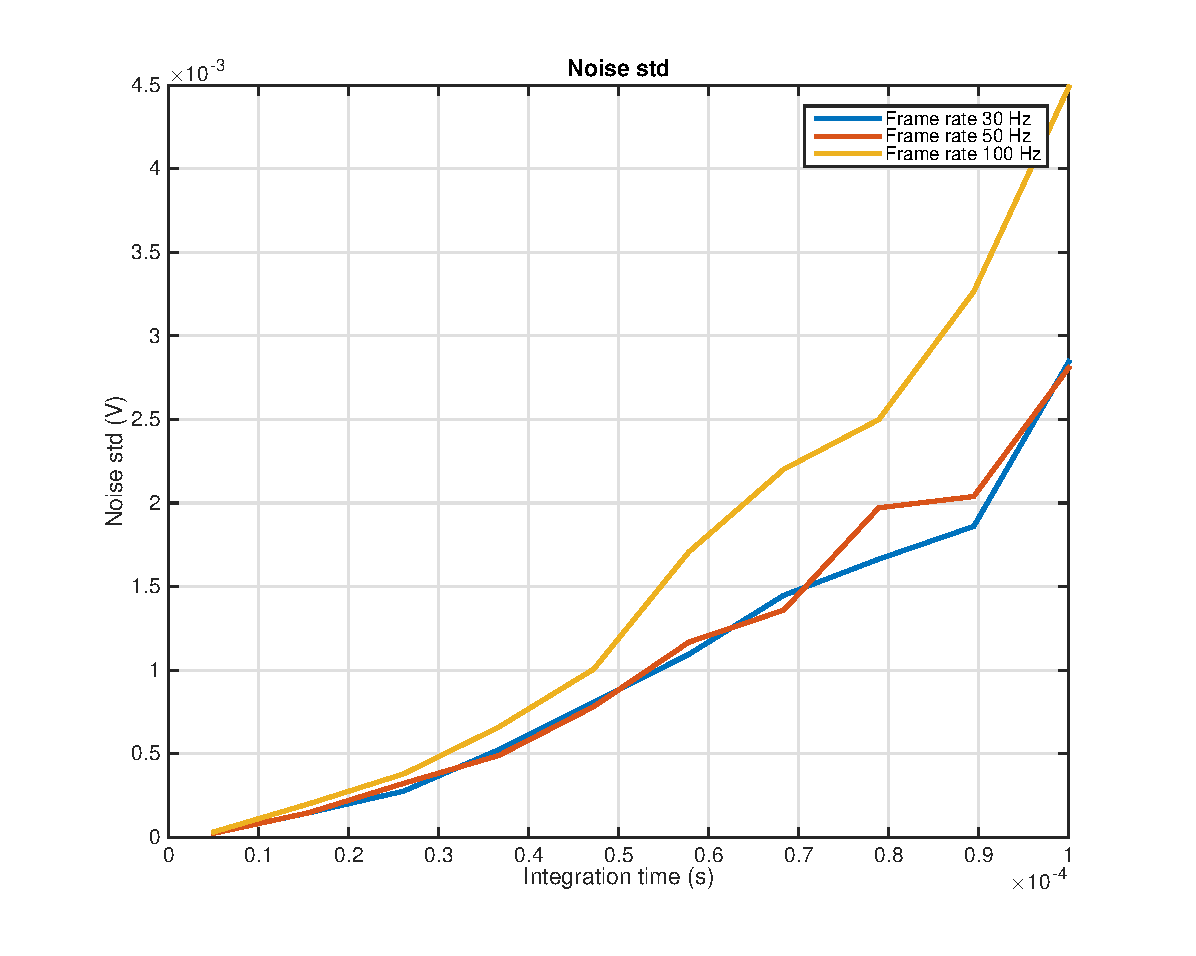
\includegraphics[scale=0.8]{gfx/STD_Function_of_Integration_Time.eps}
  \caption{Output standard deviation over integration time}
  \label{fig:std_over_time}
  \end{center}
\end{figure}


\subsection{Power spectrum of output signal}
Expertise from FLIR suggest that the power spectrum of the output signal is dependent on the frame-rate, and situated somewhere between the white and $1/f$ noise spectrum.
In order to test the accordance between this experience and the model, the power spectrum of the output signal for different frame-rates have been generated. The result can be seen in
Figure~\ref{fig:pspec}, together with a $1/f$ deterministic curve. Indeed, the output signal seems to shift from a white noise character to a $1/f$ character as frame-rates are altered.
\begin{figure}[H]
 \begin{center}
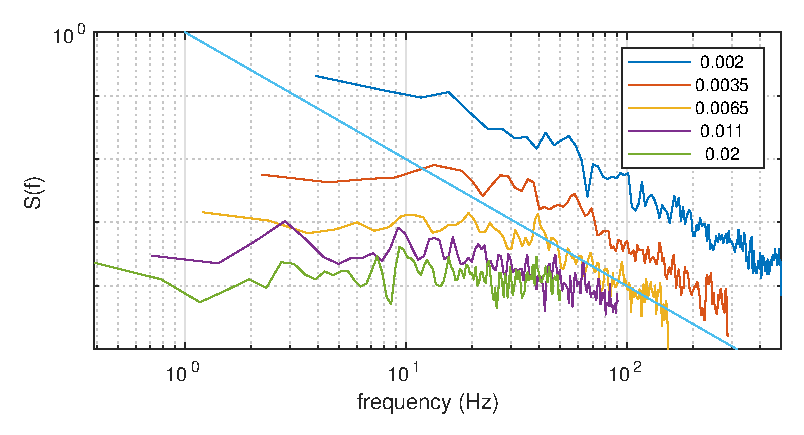
\includegraphics[scale=0.9]{gfx/pspec.eps}
  \caption{Power spectrum of output signal for different frame-rates $1/t_f$}
  \label{fig:pspec}
  \end{center}
\end{figure}

\subsection{Linearity of the output signal}
The linearity of the output signal as a function of incoming radiation effect is an assumption made during the calibration process at FLIR. The deviation of the signal from this assumption
require recalibration of the camera at regular intervals. It is therefore of interest to investigate how this linearity is affected by factors possible to influence by design. For example, FLIR suggest that the design of the bias voltage curve during integration time might be important to achieve a higher degree of linearity in the output signal. In Figure~\ref{fig:out_vs_inrad}, output signals $V_{samp}$ over incoming effect $P_{t}$ are plotted for different designs of bias voltage curve. The different bias voltage curves tested are

\begin{enumerate}
\item Constant voltage, as assumed in all previous simulations
\item Triangular voltage
\[
V(t) =
     \begin{cases}
       ax+b &\quad 0 \leq t \leq t_{i}/2\\
       cx+d &\quad t_{i}/2 \le t \leq t_{i}\\
     \end{cases}
\]
\item Bell-curve
\begin{align*}
V(t) = \frac{1}{\sqrt{2\pi \sigma^2}} e^{-\frac{(x-\mu)^{2}}{2\sigma^{2}}} \quad 0 \leq t \leq t_{i}
\end{align*}
\item Linear
\begin{align*}
V(t) = ax \quad 0 \leq t \leq t_{i}
\end{align*}
\end{enumerate}

All parameters in alternatives 1), 2), 3) are set to assure the power applied during integration time is the same as in the base case 1), and no noise is added in this simulation. Interestingly enough, a tendency towards a more linear behavior is observed for the bell shaped bias voltage curve.

\begin{figure}[H]
 \begin{center}
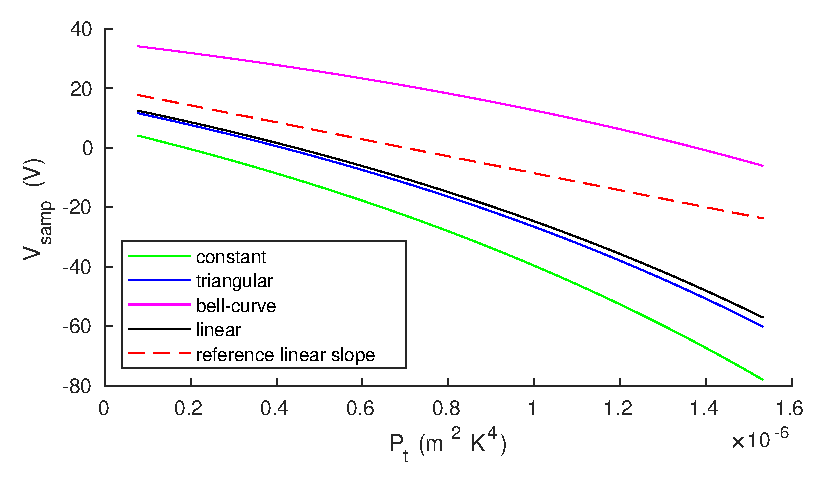
\includegraphics[scale=0.9]{gfx/out_vs_inrad.eps}
  \caption{Power spectrum of output signal for different frame-rates}
  \label{fig:out_vs_inrad}
  \end{center}
\end{figure}

\subsection{Spectrum of the output noise depending on spectrum of input noise}
The noise of the voltage is suspected to contain a component with a
$1/f$ spectrum, so called Flicker noise. It is therefore interesting
to investigate the effect of replacing the noise term in
Equation~\eqref{eq:heat_balance_equation_noise1} with a term of $1/f$
spectrum. For a detailed explanation of how such a noise term is
generated, see Section~\ref{sec:flicker-noise}. The power spectrum
of the output noise with $1/f$ noise as input is seen in
Figure~\ref{fig:power_spectrum_pink}. The output spectrum seems to be
of $1/f$ character.
%\begin{figure}[H]
%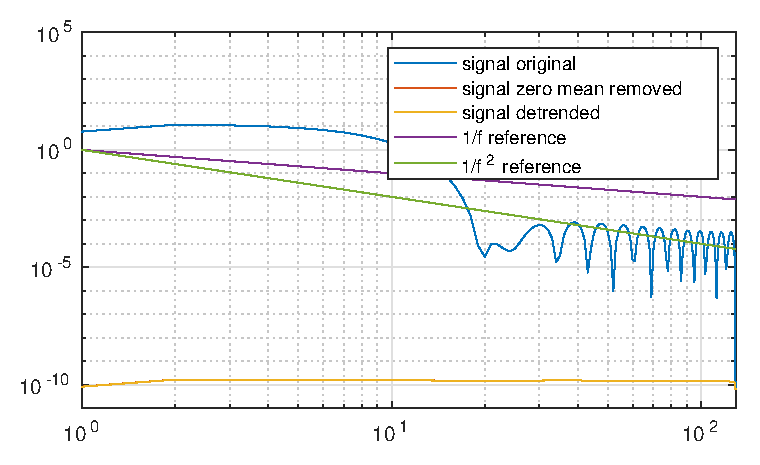
\includegraphics[scale=0.9]{gfx/spectrum_white_noise.eps}
%\caption{Power spectrum with white noise in the input. White noise in the input gives white noise in the output. \gm{Give better explanation in the caption} }
%\label{fig:power_spectrum_white}
%\end{figure}

\begin{figure}[H]
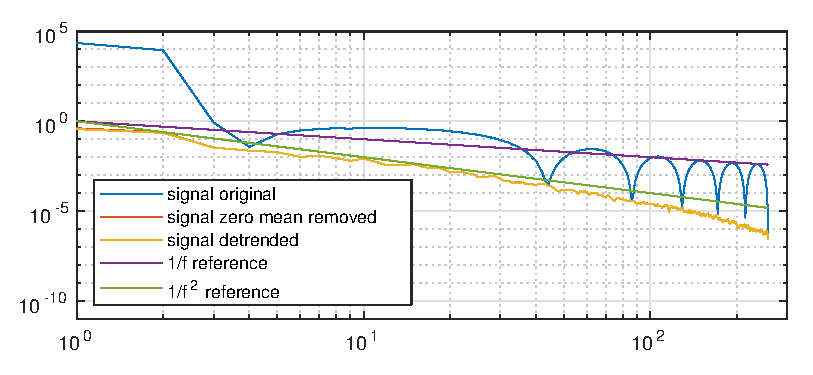
\includegraphics[scale=0.9]{gfx/spectrum_pink_noise.eps}
\caption{Power spectrum with $1/f^2$ noise in the input. $1/f^2$ noise
  in the input gives $1/f$ noise in the output.}
\label{fig:power_spectrum_pink}
\end{figure}


%%% Local Variables:
%%% mode: latex
%%% TeX-master: "main"
%%% TeX-PDF-mode: 1
%%% TeX-PDF-via-dvips-ps2pdf: 1
%%% End:
		% Carl
\section{Outlook and future extensions}				% Carl


\bibliographystyle{plain}
\bibliography{main_bib.bib}

\end{document}

%%% Local Variables:
%%% mode: latex
%%% TeX-master: t
%%% TeX-PDF-mode: 1
%%% TeX-PDF-via-dvips-ps2pdf: 1
%%% End:
